\section{Introduction}
An assistant must retain enduring interests, replace outdated instructions, and recover dormant preferences. With finite storage, historical usefulness can become a liability after a context shift: stability and plasticity are distinct requirements.

Existing systems support retrieval, reflection, consolidation, tiered storage, and updates \citep{generative,memgpt,memorybank,amem}. We isolate how per-item state changes alter the retention--adaptation balance, separately from architecture and replacement volume. Aggregate accuracy can hide dormant-knowledge loss and obsolete evidence.

With controller weights frozen, we test rate interventions on per-item state. Our contributions are:
\begin{enumerate}
\item A formulation separating immutable content, evolving state, addressing, and bounded residency, with distinct stability and plasticity objectives.
\item A hybrid evolution mechanism with explicit importance, consistency, and usage rates, event updates, and a common retention score.
\item A controlled characterization of trade-offs, replacement attribution, component roles, long horizons, and transfer failures using frozen streams and auditable trajectories.
\end{enumerate}
Code: \href{https://github.com/Nanoer-Wang/adaptive-memory-evolution}{github.com/Nanoer-Wang/adaptive-memory-evolution}.
\begin{figure}[!h]
\centering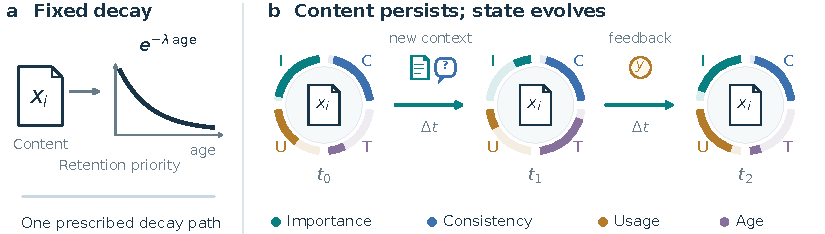
\includegraphics[width=\linewidth]{figures/concept.pdf}
\caption{Immutable content, evolving state. Fixed decay prescribes a retention path; colored arcs depict qualitative state changes, not measured or normalized values.}\label{fig:concept}
\end{figure}
